\documentclass{beamer}


\usepackage[utf8]{inputenc}
\usepackage{pgfpages}
\usepackage{xcolor}

\setbeameroption{show notes}
\setbeamertemplate{note page}[plain]
\setbeameroption{show notes on second screen=left}

\usetheme{Warsaw}
\graphicspath{ {./images/}{../images/} }

\AtBeginSection[specialframe]
{
  \begin{frame}{Table of Contents}
   \tableofcontents[currentsection]
  \end{frame}
}

\title[Kcov - a single-step code coverage tool] %optional
{Kcov - a single-step code coverage tool}

%\subtitle{A short story}

\author{Simon Kågström}

\institute
{
  Net Insight\\
  \texttt{https://github.com/SimonKagstrom/kcov}
}

%\logo{\includegraphics[height=1.5cm]{lion-logo.png}}

\begin{document}

\begin{frame}
  \titlepage
  \note{My name is Simon Kågström and I work at Net Insight as a developer of embedded software. Tonight I will present kcov, a code coverage collection and presentation tool for UNIX systems.

So let's get started!}
\end{frame}

\begin{frame}
  \frametitle{Motivation}
  \note<1->{
    \footnotesize
    I'll start with some motivation for the talk. Code coverage, as described by Wikipedia, is the degree to which the source code of a program is executed when a particular test suite executes, measured in percentage. Code coverage tools can typically show which source code lines which have been executed, and sometimes how many times they are executed.

    So let's say you're the developer of a particular piece of code, as shown on the slide. You run some tests on it, and collect code coverage to see how well your test suite actually works. NEXT.
  }

  \note<2>{
    After code coverage collection, you will get a report which looks something like this. Red lines denote executable lines which have not been executed, green lines are executed lines. White lines are non-executable lines.

    Hmm... Hang on now, why is everything between line 128 and 143 marked as non-executable? Some of you might already have identified the code in question. This is the SSL/TLS bug known as ``goto fail''. Looking at line 127, you can see that the control flow will unconditionally jump to the fail label, so lines 128 to 143 are indeed unreachable.

    Stands out pretty clear from the coverage report don't you think? Modern compilers will also issue a warning on code like this.}

  \includegraphics<1>[height=8cm]{goto_fail_no_coverage}
  \includegraphics<2>[height=8cm]{goto_fail}
\end{frame}

\begin{frame}
  \frametitle{More motivation}

  \note{We programmers should be humble people. Do you think we are?
    Anyway, why is that?  Because we all fail at times, and shoot
    ourselves in our feet. I've done this myself many times. I've
    failed with raw pointers, with shared pointers, from lambdas,
    using the Linker and so on. I've even shot myself in the foot
    using Java bytecode! So I try to be humble about my abilities, I
    know I will fail again and again.

    However, this is why I believe we need good tooling to assist
    us. Code coverage is one such tool, together with for example the
    clang sanitizers, good debuggers and so on.

    It's also the reason why good methodology is important, through
    for example test driven development and unit testing.
  }
  \begin{itemize}
  \item Programming is hard!
  \item To improve software quality, good tooling and methodology is important
  \end{itemize}
  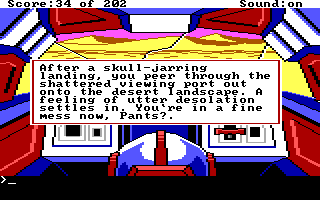
\includegraphics[width=\linewidth]{sq_skull_jarring}
\end{frame}

\begin{frame}{Outline}
  \tableofcontents
  \note{This is the outline of the rest of the talk. I will start with a short discussion of problems and limitations with traditional tools, then introduce kcov and demonstrate some of the main features.

    I will then go into a bit of details about how kcov has been implemented, and give some lessons learned in the process.

  Finally, I will discuss some other features of kcov, which are perhaps a bit less relevant on a C++ workshop.}
\end{frame}

\section{Overview}
\subsection{Some words about code coverage}
\begin{frame}{Code coverage terminology}
  \note{\footnotesize Most of you have probably encountered code coverage collection
    already, in some form. There are many variants of code coverage of
    increasing refinement, as you can see on the slide, and there are
    also others which are even more detailed and specialized.

    In most settings, MC/DC coverage is the holy grail of code
    coverage, but also something which is incredibly hard to achive in
    tests. So does kcov instrumentation support MC/DC? Unfortunately,
    it's more of an unholy grail solution, focusing on statement
    coverage like most other collectors do.

    So is code coverage collection effective? I've read a few studies,
    and the effect on software quality is mixed and unclear. That is,
    higher coverage percentage doesn't necessarily translate into
    fewer bugs. Interestingly, the type of coverage, from statement
    coverage and upwards, also doesn't make very much of a difference.

    I believe code coverage has more to offer as a test development
    tool. Especially when developing unit tests it's useful simply to
    see if your tests miss something important, and it's the area
    where I personally use it most. Pretty much daily in fact.}

  % Coverage Is Not Strongly Correlated with Test Suite Effectiveness, Laura Inozemtseva and Reid Holmes
  \begin{itemize}
  \item \textbf{Function coverage}: Functions in the program
  \item \textbf{Statement coverage}: Statements in the program
  \item \textbf{Branch coverage}: All ways through branches (if/case)
  \item \textbf{Condition coverage}: All boolean expressions evaluated to both true/false
  \item \textbf{Modified condition/decision coverage (MC/DC)}: Each decision takes every possible outcome
  \end{itemize}

  (From Wikipedia)
\end{frame}


\subsection{Problems with traditional tools}
\begin{frame}[fragile]{Problems with traditional tools}
  \note{On UNIX, the traditional way of collecting code coverage has been to use gcov for collection, and lcov for HTML presentation, if desired. The process is a bit cumbersome, as can be seen in the example below. You first need a special --coverage option, which produces extra metadata files in the build directory. After running the program, you then get data for the actual execution in the build directory.

    After this, you need to run the presentation tool, like lcov, to get actual output. If the process crashes during execution, you will lose the coverage output altogether. Gcov also doesn't gather code coverage from shared libraries.}
  \begin{itemize}
  \item gcov + lcov is a multi-step process
  \item gcov leaves droppings after compilation/running
  \item A program which crashes will not generate coverage data
  \end{itemize}
  \begin{Example}
    \begin{semiverbatim}
     \scriptsize
\$ gcc -g -Wall --coverage goto-fail.c
\$ ./a.out
\$ ls
  a.out  goto-fail.c  goto-fail.gcda  goto-fail.gcno
\$ lcov --capture --directory project-dir --output-file coverage.info
\$ genhtml coverage.info --output-directory out
    \end{semiverbatim}
  \end{Example}
\end{frame}

\begin{frame}{Instead...}
  \note{Fortunately, using kcov does away with all these disadvantages, allowing collection without special compiler options, reporting without droppings and all done in a single step. Quite a sales pitch, don't you agree? We should note here that there are other collection methods, for example via clang and obviously a set of commercial tools.}
  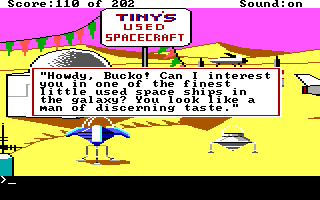
\includegraphics[width=\linewidth]{sq_ship_sales}
\end{frame}


\section{Kcov usage}
\subsection{Kcov overview}
\begin{frame}{Kcov overview}
  \begin{itemize}
  \item Kcov started as a fork of Bcov by Thomas Neumann in 2010
  \item Bcov doesn't rely on compile-time instrumentation, but instead uses debug information
  \item Bcov was a great idea, but I thought it could be improved upon
  \item<2-> Can you guess why it's called kcov?
  \item<3-> It is not related to the kernel Kcov (and predates it by many years)
  \end{itemize}

  \note{
    Kcov started as a fork of bcov, which doesn't rely on compile-time instrumentation of binaries, but instead uses the debug information present as long as you compile with -g. It can also produce lcov-like output.

    I thought bcov was a great idea, but it was still somewhat cumbersome to use, separating collection and reporting. The codebase was a bit difficult for me to follow, so I forked it instead of improving on the original project. Today I would problably not have done it that way.

    Guess the name! The original idea I had was to use kernel kprobes,
    which allows setting breakpoints on kernel code, while still
    retaining the userspace functionality. K therefore stands for
    kernel. The kernel functionality via kprobes never worked very
    well though.

    Confusingly, there is now a kcov for the kernel. The kernel kcov
    is used to more intelligently guide syscall fuzzers.}
\end{frame}

\subsection{Main features of kcov}

\begin{frame}{Main features of kcov}
  \begin{itemize}
  \item Supports collection and reporting of binaries as long as debug information is present
  \item Automatically collects coverage from shared libraries
    \begin{itemize}
      \item Both linked into the binary, and opened via \textbf{dlopen}
    \end{itemize}
  \item Collection and reporting is done in a single step
  \item Generates HTML output as well as several XML formats for integration in other environments
  \item Accumulates coverage information between runs
  \item Automatically merges multiple binaries into a combined report
    \begin{itemize}
      \item Merging of multiple reports can also be done by the tool
    \end{itemize}
  \item Works on Linux, FreeBSD and Mac OSX on x86, ARM and PowerPC
  \end{itemize}

  \note{This slide lists the main features of kcov. As I noted before,
    as long as you build with debug information, kcov has everything
    it needs for instrumentation. Optimized binaries can also be
    instrumented, but just like when debugging, this can sometimes
    give surprising results.

    Kcov also automatically detects shared libraries and instrument
    them, both from compile time and loaded during runtime.

    Unlike gcov+lcov, collection and reporting is done in the same
    command although kcov supports separating them if you collect
    coverage data from a target system where the source code isn't
    present. Output is both in HTML and various XML and Json formats
    to allow integration with external tools. More on that on the next
    slide.

    When you run the same binary multiple times, kcov will accumulate
    the coverage data as long as the binary hasn't changed. Similarly,
    when collecting from multiple binaries with the same output
    directory, kcov will create a merged report with the sources from
    all binaries.
  }
\end{frame}

\subsection{Integration with CI systems}
\begin{frame}{Integration with CI systems}
  \note{Kcov also integrates with several systems and sites for continuous integration. Jenkins has a plugin for Cobertura, normally a Java code coverage collection tool. As kcov produces XML output for Cobertura, it's easy to integrate in that environment. SonarQube is handled in a similar way.

 It also supports some popular cloud services. NEXT. It can upload directly to coveralls, which is often used together with travis-ci. Coveralls is an easy way to get fancy web stats for your project coverage. NEXT. Similarly, codecov.io is also easy to integrate, but supports kcov directly from the upstream project.

Personally, I haven't picked a favourite cloud coverage service just yet, but instead use both with travis-ci and added dual badges on github.
  }
  \begin{itemize}
  \item Jenkins and SonarQube output is generated by kcov
  \item \textcolor<2>{red}{Uploading to Coveralls.io is built-in}
  \item \textcolor<3>{red}{Uploading to Codecov.io is supported by the upstream project}
  \end{itemize}
  \includegraphics<1-2>[height=6cm]{coveralls}
  \includegraphics<3>[height=6cm]{codecov}
\end{frame}

\subsection{Python/Bash}
\begin{frame}{Python and Bash code coverage}
  \note{Kcov also supports Python and Bash coverage
    collection. Judging by the number of reported github issues, Bash
    coverage collection is surprisingly popular. Or the kcov
    implementation is just buggy!
  }
  \begin{itemize}
  \item Kcov can also collect coverage for Python and Bash
  \item For Bash and Python, line counts are reported
  \end{itemize}

  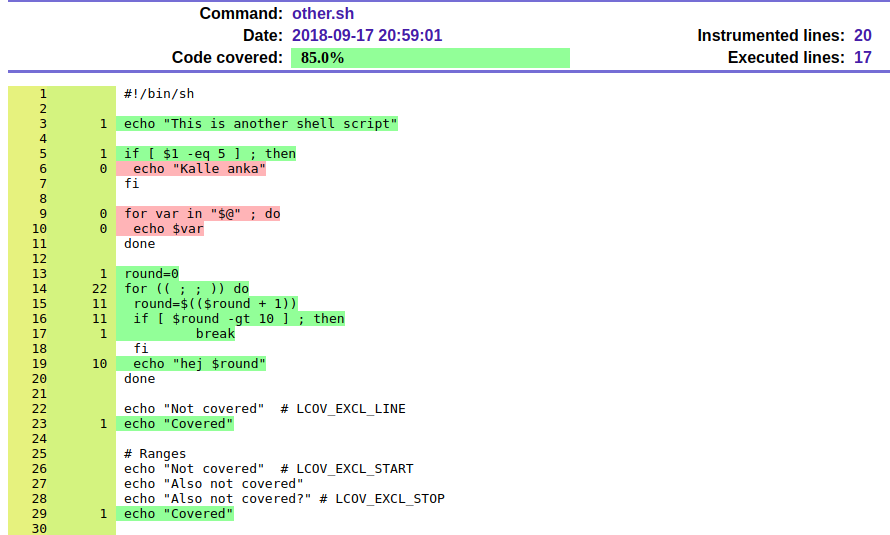
\includegraphics[width=7cm]{bash}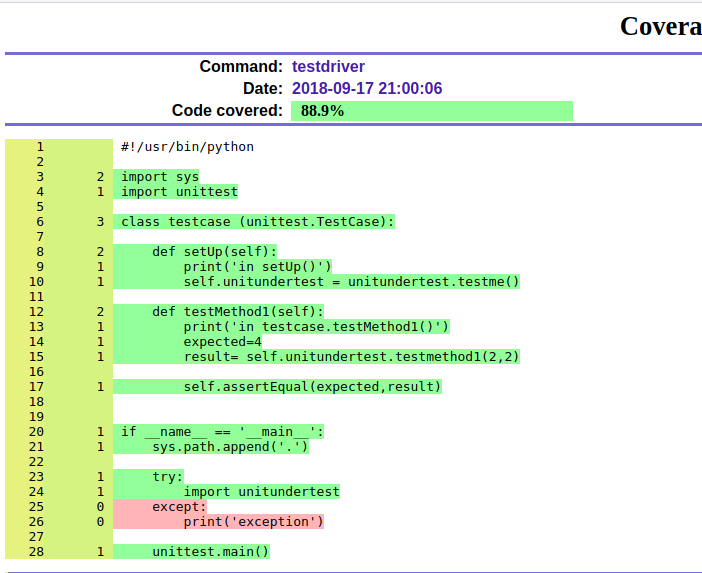
\includegraphics[width=5cm]{python}
\end{frame}

\begin{frame}{Interactive Demo!}
  \note{
      \begin{itemize}
      \item Demo: Make sure /tmp/kcov is empty

      \item kcov /tmp/kcov projects/build/kcov/target/src/kcov

      \item Show result in browser

      \item Show how a single file looks, describe 1/3, execution order etc

      \item Show file list again, note /usr/include etc

      \item Remove /tmp/kcov. All output is placed in the out-directory, so this cleans up everything from the coverage run

      \item Run kcov with --include-pattern, note that --exclude-pattern and paths also exist

      \item Run kcov unit tests, show merged report

      \item Discuss --collect-only, --report-only
    \end{itemize}
  }
  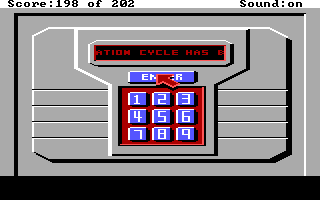
\includegraphics[width=\linewidth]{sq_keypad}
\end{frame}

\section{How kcov works}

\subsection{Elves, dwarves and breakpoints}
\begin{frame}{Dwarf stabs Mach-O Elf}
  \note{\footnotesize Lets start with an overview of technologies used
    by kcov. Binaries in Linux are nowadays almost always stored in
    the ELF binary format. ELF binaries contain sections which contain
    code, data, constants, relocation information and so on. Where
    relevant, the sections contain a memory address where the code or
    data is loaded into memory during execution.

    On Mac OS X, Mach-O is used as the binary format, and functions in
    pretty much the same way as ELF. Windows has some other format.

    The most important of these for kcov is Dwarf, however. Dwarf is a
    format for debug information, and is related but independent from
    the binary formats. Dwarf sections are present in both ELF
    binaries, and Mach-O dittos and contain information needed by
    debuggers. For example, the mapping between source lines and
    addresses is needed when you set a breakpoint on a source line,
    variable type information when you print variables and so on.

    I guess you've noted by now that the world of binary file formats
    and debug information is full of funny names. Stabs is an older
    format for debug information, seldomly used today.

  We'll continue with how kcov uses these on the next slide.}

  \begin{itemize}
  \item \textbf{ELF} is a binary format used on many Unices
    \begin{itemize}
    \item Both for object files, shared libraries and executable files
    \item Contains the code, data, constants and relocation information
    \end{itemize}

  \item \textbf{Mach-O} is the binary format used on Mac OS X
  \item \textbf{Dwarf} is a format for debug information
    \begin{itemize}
    \item Contains the mapping between source lines and addresses
    \item Type information for variables etc
    \end{itemize}
  \end{itemize}

\end{frame}

\begin{frame}[fragile]{Instrumenting binaries with kcov}
  \note{
    Kcov relies on Dwarf debug information to set a breakpoint on each executable line in the program. The debug information contains records of file:line to address mappings, which is exactly what kcov needs. NEXT. In the disassembly output, you can see this as the instructions marked in red, which correspond to DWARF entries.
% Disassembly here
    
    Kcov starts the program in stopped state, sets all breakpoints and then lets the program continue again. On each executed breakpoint, kcov marks the file:line pair as executed, removes the breakpoint and lets the program continue again. That's the basic way kcov works.
  }
  \begin{itemize}
    \item DWARF contains file:line to address records, which kcov uses to set breakpoints
    \item<3-> So how are breakpoints set on Linux?
  \end{itemize}
  \begin{Example}
    \begin{semiverbatim}
      \scriptsize
 124:     return (void*)op\_create(RPAR);
400ff7:       \textcolor<2>{red}{bf 30 00 00 00}          mov    \$0x30,\%edi
400ffc:       e8 1f 05 00 00          callq  401520 <op\_create>
401001:       e9 20 ff ff ff          jmpq   400f26 <ts\_next\_token+0x46>
401006:       66 2e 0f 1f 84 00 00    nopw   \%cs:0x0(\%rax,\%rax,1)
40100d:       00 00 00
 125: p\_state->last\_token\_is\_od = 0;
401010:       \textcolor<2>{red}{c7 43 08 00 00 00 00}    movl   \$0x0,0x8(\%rbx)
 126: return (void*)op\_create(op);
401017:       \textcolor<2>{red}{bf 04 00 00 00}          mov    \$0x4,\%edi
40101c:       e8 ff 04 00 00          callq  401520 <op\_create>
   \end{semiverbatim}
   \end{Example}
 % Disassembly
  % file:line -> addr
  % Cleared once it has been executed
\end{frame}

\begin{frame}[fragile]{How does kcov know where to set the breakpoint, really?}

  \note{
  }
  \begin{itemize}
  \item What's in the ELF binary
  \item PIEs, sections loaded into memory
  \end{itemize}
 % Disassembly
  % file:line -> addr
  % Cleared once it has been executed
\end{frame}

\subsection{Implementation quirks on different architectures}

\begin{frame}[fragile]{kcov on Linux, FreeBSD and Mac OSX}
  \note{\footnotesize There is no fully standardized way of setting and controlling breakpoints on UNIX. The ancient ptrace is typically used for this, through PEEKTEXT/POKETEXT options. The original bcov implementation is the base for the Linux implementation, but Alan Somers have more recently extracted the OS-dependent parts and ported Kcov to FreeBSD. On Linux and FreeBSD, libelf and elfutils is used for parsing binaries.

OSX works in an entirently different way though. The key difference between OSX and Linux/FreeBSD is that OSX uses it's own binary format, Mach-O. So we now have Dwarves, Elves and Mach-O. For ELF, we have libelf to do the parsing, but Apple doesn't publish a library for Mach-O. I therefore opted on a simpler solution on OSX. The LLDB debugger comes with the development environment on OSX, and it conveniently offers a nice C++ API.

So on OSX, the entire parsing, process control and breakpoint setting is only 486 lines of code. The disadvantage with the LLDB implementation is that it's significantly slower than using regular ptrace. During normal debugging, you typically don't set tens of thousands of breakpoints!

Ptrace is quite messy to work with. The code snippet shown is for dumping the register file when the program stops at a breakpoint. As you can see, it's not standardized between architectures, not to mention between OSes. When you have the registers, kcov needs to know the program counter, which is one of the entries in the register file. Obviously in different positions on different architectures! The easiest way to find it has been to look in GDB or the Linux kernel source code.

% Not automatically portable
  }
    \begin{itemize}
    \item ptrace is a truly archaic interface, and pretty non-portable
    \item libelf is also interesting: \textbf{elf\_version} must be called at program start!
    \item Mac OSX has been implemented using the LLDB debugger as a library
    \end{itemize}
  \begin{Example}
    \begin{semiverbatim}
      \scriptsize
static long getRegs(pid\_t pid, void *addr, void *regs, size\_t len)
\{
#if defined(\_\_aarch64\_\_)
    struct iovec iov = \{regs, len\};
    return ptrace(PTRACE\_GETREGSET, pid, (void *)NT\_PRSTATUS, &iov);
#else
    return ptrace((\__ptrace\_request ) PTRACE\_GETREGS, pid, NULL, regs);
#endif
\}
    \end{semiverbatim}
  \end{Example}
\end{frame}

\begin{frame}{Design}
  \note{
    \footnotesize
    Kcov is written in C++, but unfortunately it's C++03, so a bit unmodern for these kinds of meetings! I'll just shortly discuss the kcov design a bit.

The design revolves around a set of abstract interfaces, as show on the figure and through heavy use of the observer pattern. Binary files are parsed via the IFileParser interface. Binary execution is handled through the IEngine interface, and output is handled via the IWriter interface.

Control is handled through the collector, which receives file/line to address mappings from the file parser. The collector will then set breakpoints, execute the program, and collect breakpoint hits through the engine. The reporter receives and memorizes executed lines and reports them to the writers, which produces the output. Pretty simple, don't you think?

The design was originally made to accomodate ELF and ptrace, and the only true File parser is the Elf parser. When kcov is used with Python, bash or indeed on OSX via LLDB, parsing and execution is kept together, so these implement both the engine and the file parser interfaces.}
  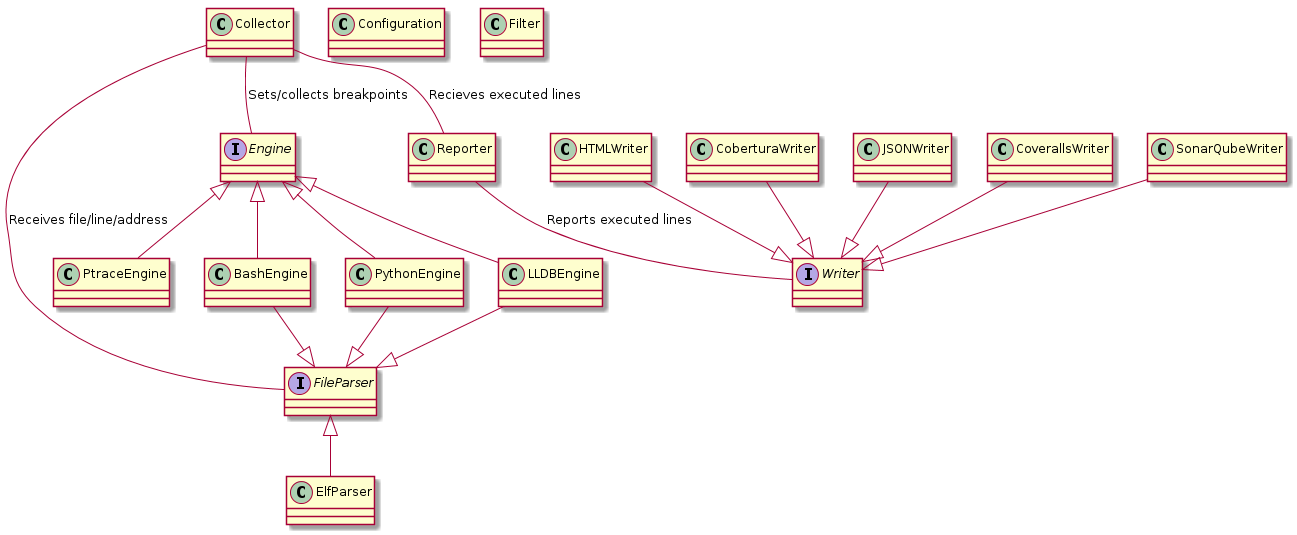
\includegraphics[width=\linewidth]{design}
\end{frame}

\subsection{ELF/Dwarf implementation quirks}
\begin{frame}{So are there any interesting bugs?}
  \note{So are there any interesting bugs affecting kcov?}
  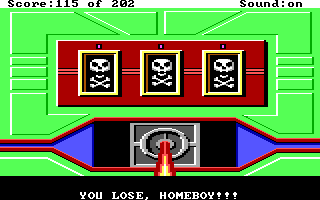
\includegraphics[width=\linewidth]{sq_slotmachine}
\end{frame}

\begin{frame}[fragile]{Dwarf quirks}
  \note{
    \footnotesize
    There are some interesting quirks and bugs concerning Dwarf usage in Linux. The most irritating and interesting one is when the file:line to address entries contain invalid entries. We again have the disassembly output you saw before. NEXT. However, if you look at the second entry marked in red here, you see that it points into the middle of an instruction.

    This is possible on x86 since it has variable instruction length, so an instruction can start on any byte address. Now, a breakpoint on x86 is simply a special instruction, encoded with a single byte, 0xcc hex. Setting a breakpoint therefore means overwriting the start of the instruction you want to break at with 0xcc. But if 0xcc is written into the middle of an instruction, you either get an invalid instruction, or even worse, a valid but unintended instruction.

    kcov works around this by simply disassembing the entire program, and discarding Dwarf entries which doesn't point to the start of an instruction. This is somewhat expensive, so it's only enabled with an option. On architectures which have a fixed instruction length, it instead discards entries which are unaligned to natural instruction borders.}
  \begin{itemize}
    \item Dwarf generation on Linux is sometimes buggy, containing invalid entries
  \end{itemize}
  \begin{Example}
    \begin{semiverbatim}
      \scriptsize
 124:     return (void*)op\_create(RPAR);
400ff7:       \textcolor<2>{red}{bf 30 00 00 00}          mov    \$0x30,\%edi
400ffc:       e8 1f 05 00 00          callq  401520 <op\_create>
401001:       e9 20 ff ff ff          jmpq   400f26 <ts\_next\_token+0x46>
401006:       66 2e 0f 1f 84 00 00    nopw   \%cs:0x0(\%rax,\%rax,1)
40100d:       00 00 00
 125: p\_state->last\_token\_is\_od = 0;
401010:       c7 43 \textcolor<2>{red}{08 00 00} 00 00    movl   \$0x0,0x8(\%rbx)
 126: return (void*)op\_create(op);
401017:       \textcolor<2>{red}{bf 04 00 00 00}          mov    \$0x4,\%edi
40101c:       e8 ff 04 00 00          callq  401520 <op\_create>
   \end{semiverbatim}
   \end{Example}
\end{frame}
  % file:line maps to an invalid address
  % ptrace: Does not set breakpoints, modifies memory
  % ptrace is not recursive, can't strace kcov
  % When a process stops, you need to dump the register file and find the PC. This is
  % architecture and OS dependent

\subsection{Python and Bash coverage collection}

\begin{frame}{So how does Python and Bash work?}
  \begin{itemize}
  \item Bash has a \textbf{PS4} environment variable, which can be used to trace execution
  \item Python has a trace function which can be controlled via \textbf{sys.settrace}
  \item kcov needs to know what lines are ``executable'' and not, also in this setting
    \begin{itemize}
    \item Easy in Python
    \item \textit{Very} tricky in Bash. Heredocs etc
    \end{itemize}
  \end{itemize}
\end{frame}

\subsection{System mode}
\begin{frame}{System mode}
\end{frame}

\begin{frame}{Questions and comments!}
  \footnotesize
  (Images from \url{http://www.falselogic.net/LetsPlay/SpaceQuest.html})
  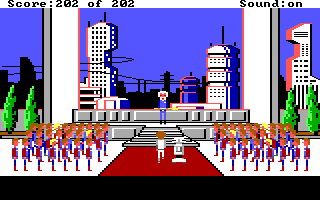
\includegraphics[width=\linewidth]{sq_final}
\end{frame}

\end{document}


%- How kcov works

%  - A bit about how gcov works

%  - Breakpoints

%  - Differences between OSX and Linux/FreeBSD

 % - Complain a bit about elf_version/libdwarf etc.


% - What about speed?
